\documentclass{standalone}
\usepackage{tikz}
\begin{document}
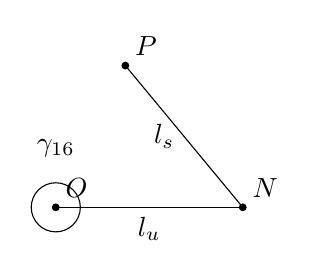
\begin{tikzpicture}[scale=0.6]
  \filldraw (0.0, 0.0) circle (2pt) node[above right] {$O$};
  \filldraw (3.9577, 0.0) circle (2pt) node[above right] {$N$};
  \filldraw (1.4731, 3.0) circle (2pt) node[above right] {$P$};
  \draw (0.0, 0.0) -- (3.9577, 0.0) node[midway, below] {$l_u$};
  \draw (1.4731, 3.0) -- (3.9577, 0.0) node[midway, left] {$l_s$};
  \draw (0.0, 0.0) circle (0.5196) node[above=0.5196cm] {$\gamma_{16}$};
\end{tikzpicture}
\end{document}